% Section 3.4.x  Realistic logistics layouts.  Written for the final report from
% the warehouse engineering record (aws-robomaker-small-warehouse-world/
% MEMORY_CLAUDE/README.md, sections 28-28e) and the generator sources; it is not
% a fragment of the retired minor report, which predates these worlds.
\subsection{Realistic logistics layouts}
\label{sec:realistic-worlds}

\textbf{Status: \status{implemented} after the reporting cutoff (6 October 2026);
no result slot in \cref{chap:results} uses these worlds yet.} The object
arrangements of \cref{sec:environments-datasets} were built as controlled
stimuli: props distributed over the floor, props confined to the wall region,
and props shuttling back and forth along fixed segments. None of them is laid
out as a warehouse is laid out, and none of their dynamic props does anything a
warehouse vehicle does. Two further worlds were therefore generated from the
warehouse-design literature collected under \repo{docs/references/warehouse/},
whose common prescription is a chain of zones---receiving, storage, picking,
packing, dispatch---served by cross-aisles, with the fast-moving goods nearest
the docks, bulk storage at the back or side, and offices and equipment charging
out of the flow \cite{asean2019warehouse,mecalux2024layout}. The two
canonical flow shapes of that literature are both provided:

\begin{itemize}
  \item \textbf{U-shape flow}, \repo{worlds/small_warehouse_dynamic/small_warehouse_dynamic_realistic_nofloortexture.world}:
    receiving and dispatch docks on the same (north) wall with the management
    office between them, the fast pick faces nearest the docks, rack storage in
    north--south aisles, picking and packing east, block storage west, and the
    charging area, empty-pallet store and general office along the south wall.
  \item \textbf{I-shape (through) flow}, \repo{..._realistic_nofloortexture_01.world}:
    receiving docks on the north wall and dispatch docks on the south wall, rack
    storage in the middle, the pick faces between storage and dispatch, packing
    beside dispatch, block storage west and both offices on the east wall, so
    that goods cross the building in one direction.
\end{itemize}

Both are written by \repo{script/make_realistic_world.py} (\texttt{--layout u}
or \texttt{i}) from parametric tables and are never edited by hand. Everything
that is not the object arrangement is held fixed: the same \SI{41.28}{\metre}
shell, the same plain (\texttt{nofloortexture}) floor, lights, physics
configuration (\cref{tab:physics-setup}) and robot spawn. The only change to
the shell is a regenerated wall model carrying dock-door openings, since the
stock wall's geometry is frozen in its mesh. The controlled factors of
\cref{tab:controlled-factors} are therefore unchanged; the new worlds add two
levels to the \emph{prop or route arrangement} factor and, as explained below,
make \emph{scene dynamics} a within-arrangement factor for the first time.

\begin{figure}[p]
  \centering
  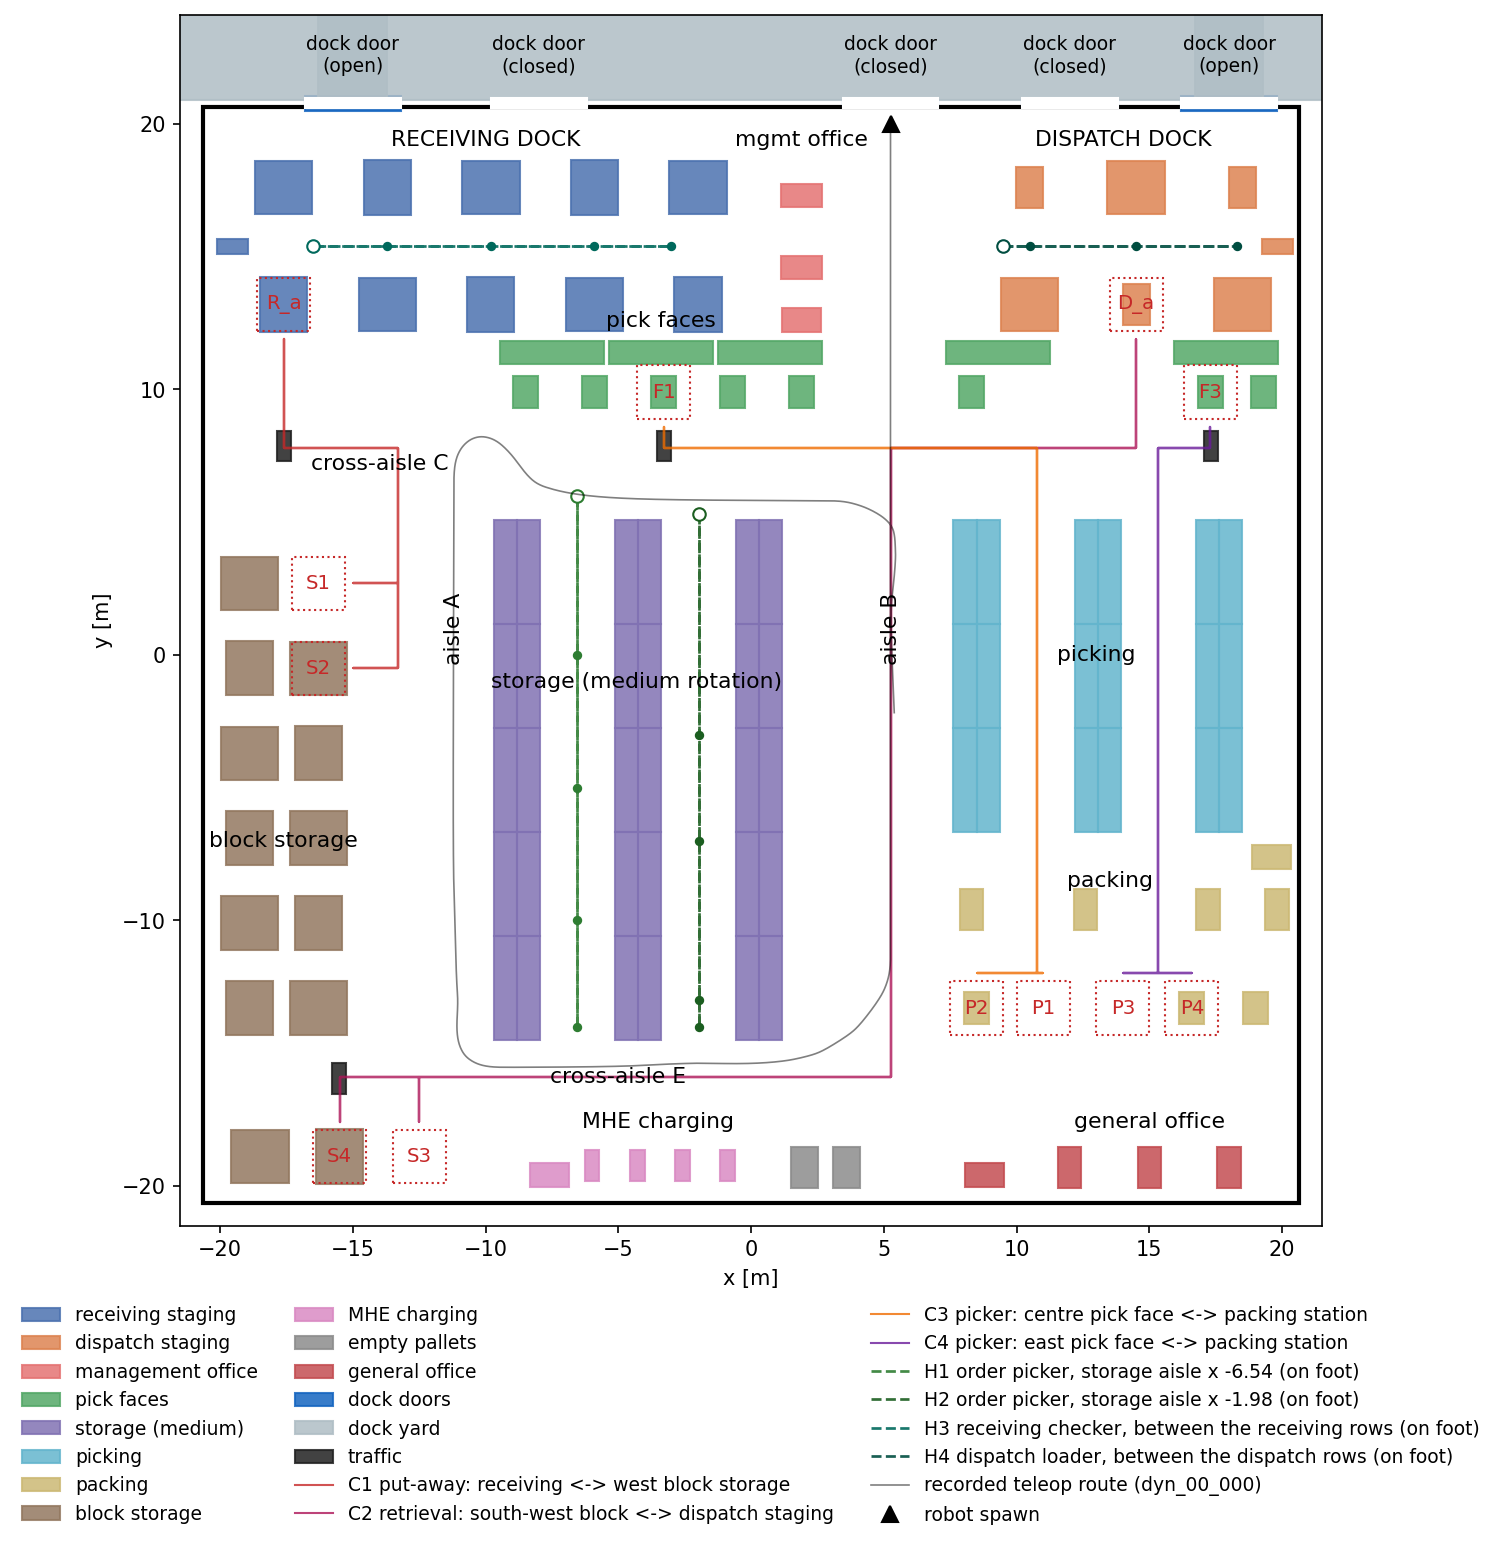
\includegraphics[width=0.92\textwidth]{figures/plan_realistic_u.png}
  \caption[Plan of the U-shape realistic world: zones, carrier jobs and dock doors, drawn by the generator from the tables that write the world file.]{Plan of the U-shape realistic world, drawn by the generator from the
  same tables that write the world file. Filled rectangles are object footprints
  coloured by zone; dotted red boxes are the exchange slots the carrier jobs pick
  from and drop on (labels \texttt{R\_a}, \texttt{S1}\ldots\texttt{P4}); the
  coloured polylines are the four carrier routes; the dashed green lines are
  the routes of the four people on foot, with a dot at each place they stop and
  an open circle where they start; the grey trace is the
  ground-truth route of \repo{dataset_dynamic_nofloortexture_00_000}, which the
  main aisles A and B and cross-aisles C and E were placed to keep drivable. The
  band above the north wall is the dock yard with the two docked trailers.}
  \label{fig:realistic-plan-u}
\end{figure}

\begin{figure}[p]
  \centering
  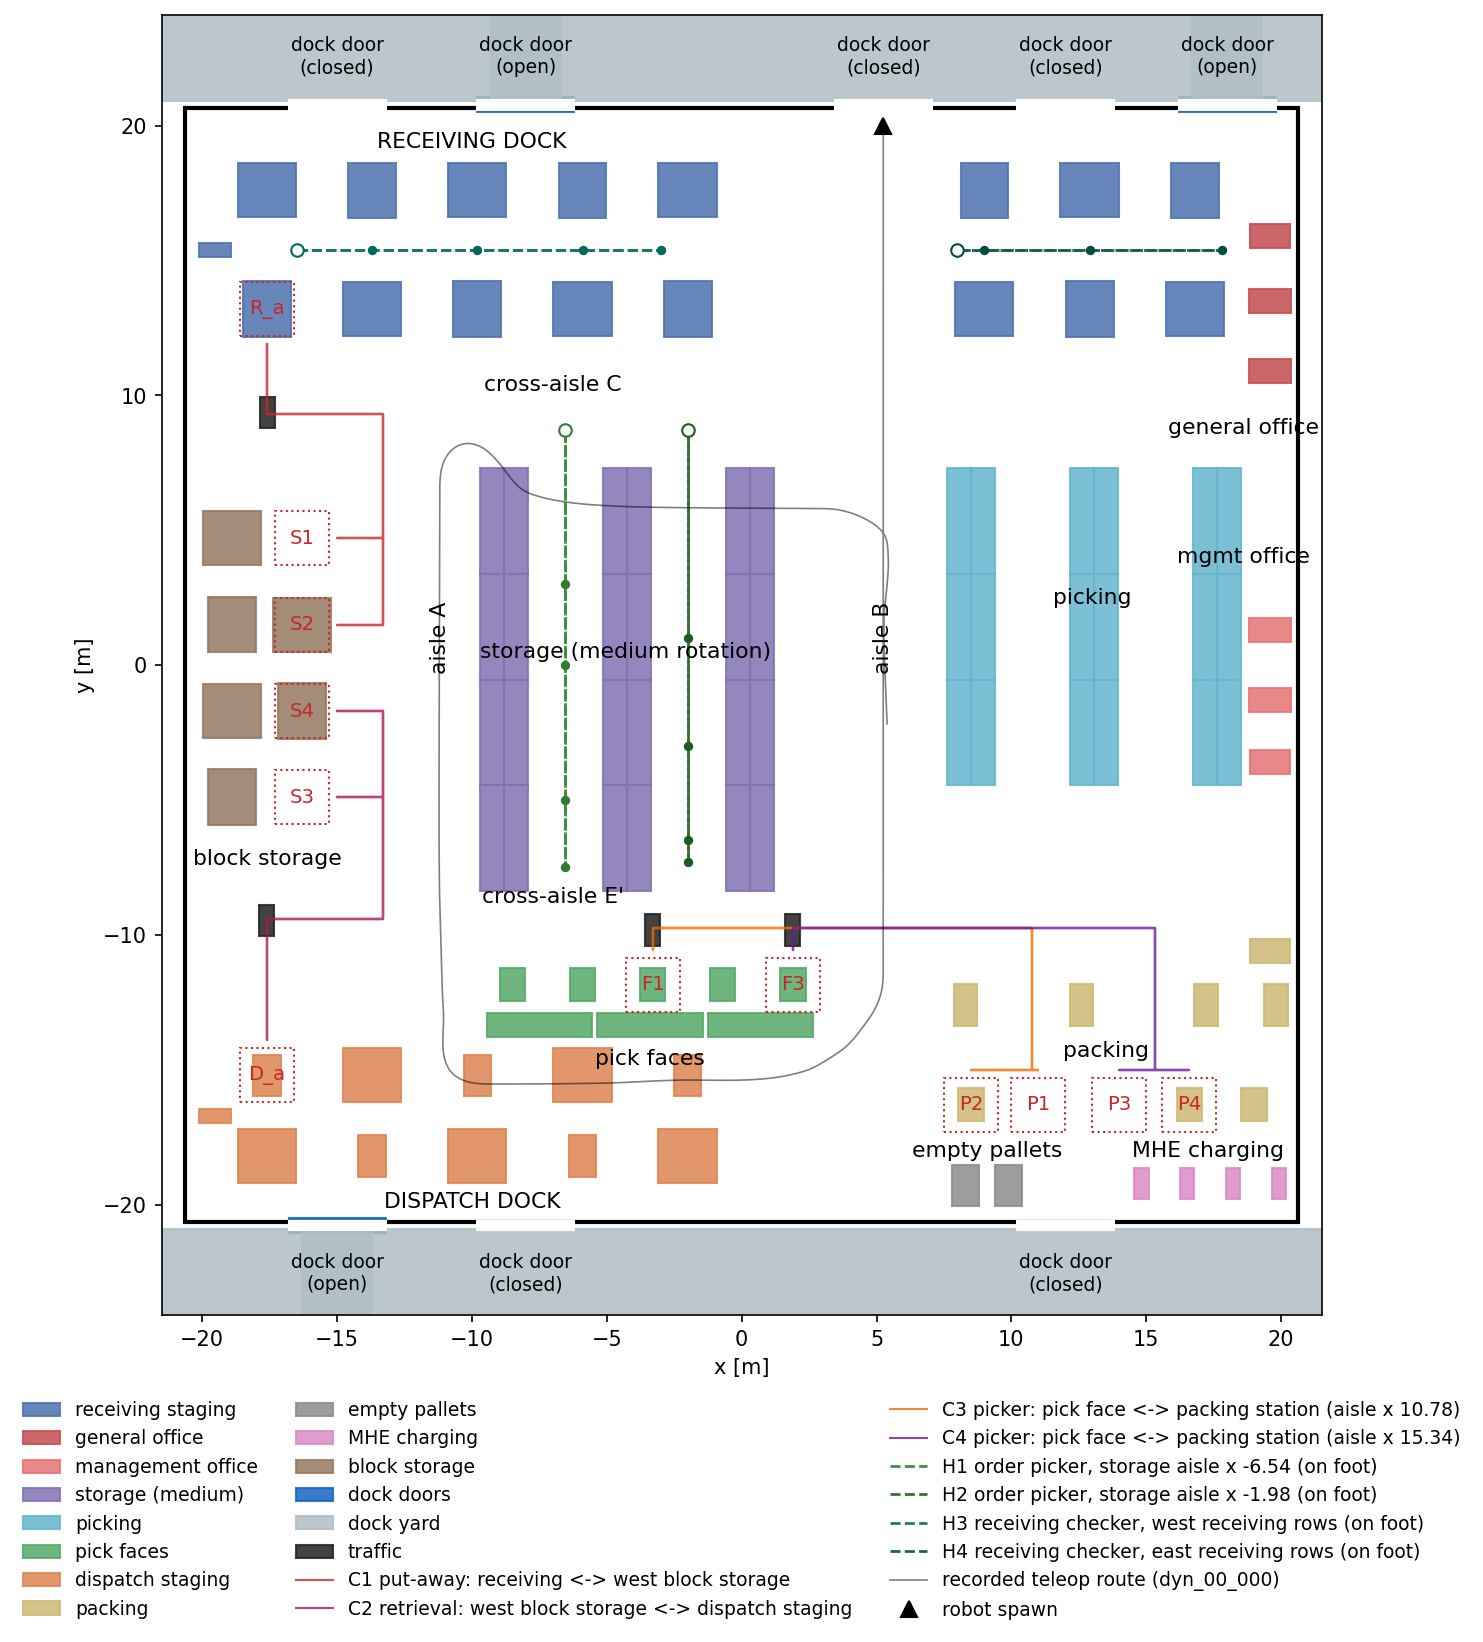
\includegraphics[width=0.88\textwidth]{figures/plan_realistic_i.png}
  \caption[Plan of the I-shape realistic world, same conventions as the U-shape plan; dispatch docks are on the south wall.]{Plan of the I-shape realistic world, with the conventions of
  \cref{fig:realistic-plan-u}. Receiving docks are on the north wall and dispatch
  docks on the south wall; the pick faces sit between the storage racks and
  dispatch, and both offices are on the east wall because with docks on opposite
  walls the office cannot lie between reception and dispatch. The recorded
  teleop route (grey) crosses the storage racks here and is \emph{not} drivable
  in this layout.}
  \label{fig:realistic-plan-i}
\end{figure}

\paragraph{Zones and contents.} \Cref{tab:realistic-zones} lists what each
zone holds. Aisles are \SI{3.0}{\metre} between zones and \SI{2.8}{\metre}
between rack rows; pallet pitches are \SIrange{3.2}{4.0}{\metre}, widened from
the \SI{2.4}{\metre} of a stock bay so that a loaded pallet jack has the
\SI{2.6}{\metre} of swing room it needs to turn. The dock doors are
\SI{3.6}{\metre} by \SI{4.5}{\metre} openings in the wall; a closed door is a
roll-up panel in the wall thickness, an open door shows a docked
\SI{13.6}{\metre} semi-trailer and a yard slab, so that a camera looking out
through it sees a trailer interior and tarmac rather than the sky colour. The
U-shape world has five doors on the north wall (two open), the I-shape five on
the north and three on the south (three open in all).

\begin{table}[htbp]
\centering
\caption[Zones of the two realistic worlds and the number of object instances each holds.]{Zones of the two realistic worlds and the number of object instances
each holds, counted from the generator's tables. ``Inside'' excludes the dock
doors, trailers and yard, which lie in or beyond the wall line. The four
carriers are the pallet jacks the traffic plugin drives.}
\label{tab:realistic-zones}
\small
\begin{tabularx}{\textwidth}{>{\raggedright\arraybackslash}p{0.26\textwidth}>{\raggedright\arraybackslash}Xrr}
\toprule
Zone & Contents & U-shape & I-shape \\
\midrule
Receiving staging & pallet loads in two rows, one parked jack & 11 & 17 \\
Dispatch staging & pallet loads in two rows, one parked jack & 7 & 11 \\
Pick faces & east--west shelves with totes in front & 13 & 8 \\
Storage, medium rotation & three double rack rows & 30 & 24 \\
Picking & three double rack rows & 18 & 18 \\
Packing & four desks, totes, bin & 8 & 8 \\
Block storage & floor-stacked pallets, one empty cell per job & 13 & 6 \\
Management office & two desks, bin & 3 & 3 \\
General office & desks, bin & 4 & 3 \\
MHE charging & parked pallet jacks, bin & 5 & 4 \\
Empty pallets & stacks & 2 & 2 \\
Carriers (traffic) & pallet jacks on jobs & 4 & 4 \\
People on foot (actors) & order pickers and dock checkers; not objects, not counted below & 4 & 4 \\
\midrule
Inside the walls & & 118 & 108 \\
Dock doors, trailers, yard & & 8 & 13 \\
Total object instances & & 126 & 121 \\
\midrule
Baked occupancy (\si{\percent} of cells) & & 20.7 & 19.1 \\
\bottomrule
\end{tabularx}
\end{table}

\paragraph{Traffic as jobs, not shuttles.} The dynamic props of the earlier
family move back and forth along a segment. In the realistic worlds the moving
objects are four pallet jacks on logistics jobs, driven by a second
world-level Gazebo system, \repo{gz_kinematic_trajectory/LogisticsScheduler.cc}:
a carrier drives to a load, takes it onto its forks (the load's pose relative to
the carrier is captured at pick-up and held rigidly through every turn),
carries it through the aisles, sets it down on a target slot and goes for the
next. Two jacks move pallets between receiving, block storage and dispatch; two
move totes between the pick faces and the packing desks. Each job is a
six-move rotation over two loads and three slots that returns to its starting
state, so it loops indefinitely and no drop ever lands on an occupied slot.
Carriers move at \SIrange{1.2}{1.3}{\metre\per\second}, turn in place at
\SI{1.5}{\radian\per\second}, spend \SIrange{4}{5}{\second} on each pick or
drop, and carry the load \SI{1.3}{\metre} ahead of the body. Slots are entered
head-on and left in reverse, as a real jack does; the first design spun the
loaded jack on the spot and swung the pallet into the neighbouring loads. The
mechanism is the same kinematic pose command used by the earlier dynamic props,
so the fidelity caveat of \cref{sec:sim-fidelity} is unchanged: the vehicles
cost no physics and offer no collision response if the robot drives into them.

Before a world is written the generator proves it: every static pair is at
least \SI{0.25}{\metre} apart (rack runs excepted), every job's slot
bookkeeping is simulated, and for every leg and every turn the swept box of the
carrier plus its load is checked against every object not in that carrier's
own job. Both worlds pass with every clearance positive, the tightest being
\SI{0.10}{\metre} at a packing-desk turn in each. Carriers can still cross one
another briefly at an aisle intersection; that is a visual overlap, not a path
conflict, and it is accepted.

\paragraph{People on foot.} A warehouse floor also has people on it, and they
are the dynamic objects a visual pipeline finds hardest: articulated,
self-occluding and close to the camera. Each world therefore carries four
walking people (added 9 October 2026), written as Gazebo \emph{actors}: the
stock Fuel walking-person skin, packaged as
\repo{models/aws_robomaker_warehouse_Person_01}, animated with a walk clip
between stops and a stand clip at them, on a scripted closed route with one
spline per leg so that legs stay straight in the aisles. The roles follow the
same references as the layout and the Eaton case study
\cite{mir2024eaton}: two order pickers, one per storage aisle, who walk the
aisle, stop at bays for six seconds and turn at the ends; and two dock
checkers who walk the lane between the staging rows and stop at loads---in the
U-shape one at receiving and one at dispatch, in the I-shape one on each
receiving group. Walking speed is \SIrange{1.1}{1.2}{\metre\per\second}, starts
are staggered, and the number was kept small deliberately: four people on
\SI{1704}{\metre\squared} with four vehicles is a working floor, not a crowd.
People keep out of the vehicle lanes by construction. The generator sweeps a
\SI{0.7}{\metre} person box along every leg and checks it against the statics
(at least \SI{0.25}{\metre}), the carrier corridors and turn sweeps (no
overlap) and the other people; the tightest clearances are
\SI{0.59}{\metre} to a static and \SI{0.34}{\metre} to a carrier sweep. The
pickers turn at the aisle mouths, which places them in view of a robot driving
the cross-aisle. Actors have no collision geometry and no physics: nothing can
bump into them, the occupancy bake does not see them, and the static twins
omit them. One limitation matters for scoring: a scripted actor's animated
pose is computed on the rendering side and is not written back to the entity
state, so \repo{/world/default/pose/info} reports a person at its initial
pose throughout. The script is deterministic, so the pose is instead
evaluated from the world file and the simulation clock by
\repo{script/people_script.py}, which the 2-D viewer uses to draw the people
(linear between the \SI{2}{\metre} waypoints, within \SI{0.2}{\metre} of the
rendered spline). Projecting a detector ground truth from it is not yet
implemented, so Experiment~2 cannot yet score the people and Experiment~3
sees them only as unlabelled motion.

\paragraph{Static twins.} For each layout a static world,
\repo{worlds/small_warehouse_static/small_warehouse_static_realistic_nofloortexture.world}
and its \repo{..._01.world} counterpart, is derived by \repo{script/make_static_world.py}: every object is marked static
and the traffic plugin removed, with nothing else changed. This is the
methodological point of the family. In the earlier worlds the static
arrangement (\texttt{\_01}) and the dynamic arrangements (\texttt{\_00} to
\texttt{\_02}) differ in geometry as well as in motion, so a static-versus-dynamic
comparison on them is confounded by the arrangement. A realistic world and its
twin share every footprint and differ only in whether four vehicles move.

\paragraph{Occupancy truth and routes.} The baked grids
(\cref{fig:realistic-maps}) are produced exactly as those of
\cref{fig:warehouse-maps}, with the moving carriers and their loads rasterised
at their $t=0$ pose, which is where the static twin holds them permanently. The
closed dock doors appear as a one-cell line in the wall; the open ones are gaps
onto the yard. The U-shape world keeps the main aisles A ($x\approx-11.2$~m)
and B ($x=5.25$~m, the dock lane the robot spawns in) and the cross-aisles C
and E where the recorded teleop route of
\repo{dataset_dynamic_nofloortexture_00_000} drove, which that route clears
by at least \SI{0.69}{\metre}; the other three recorded routes wander into what
is now receiving staging. The I-shape world fits none of the recorded routes
and needs new recordings.

\begin{figure}[htbp]
  \centering
  \begin{minipage}[t]{0.48\textwidth}
    \centering
    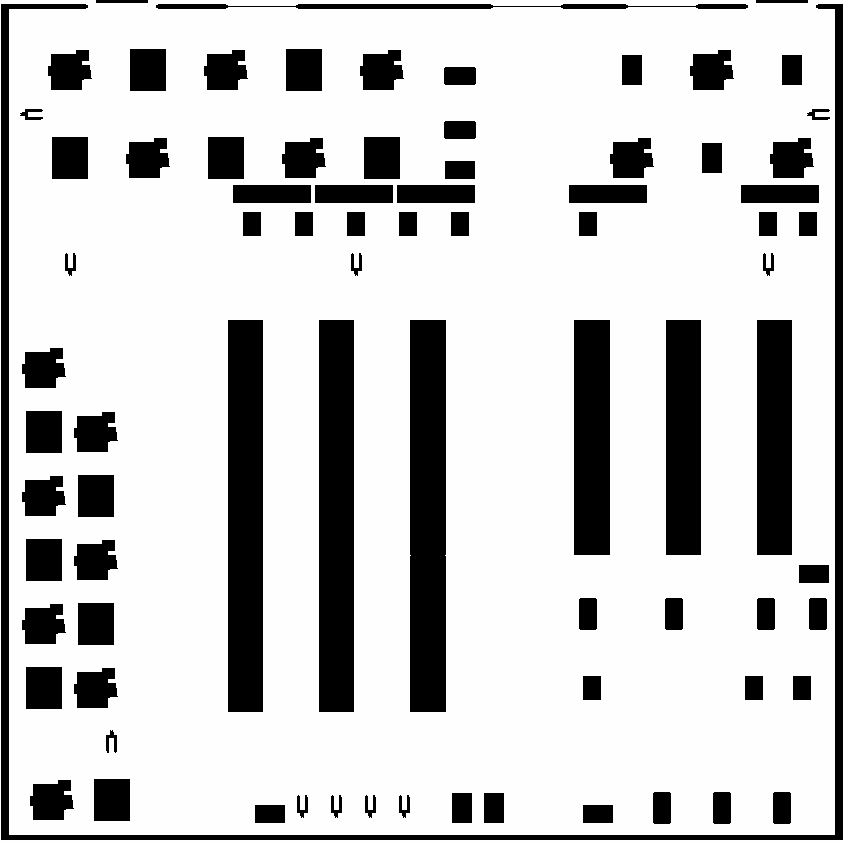
\includegraphics[width=\textwidth]{figures/warehouse_realistic_u.png}\\[0.4ex]
    {\footnotesize (a) U-shape, \SI{20.7}{\percent} occupied}
  \end{minipage}\hfill
  \begin{minipage}[t]{0.48\textwidth}
    \centering
    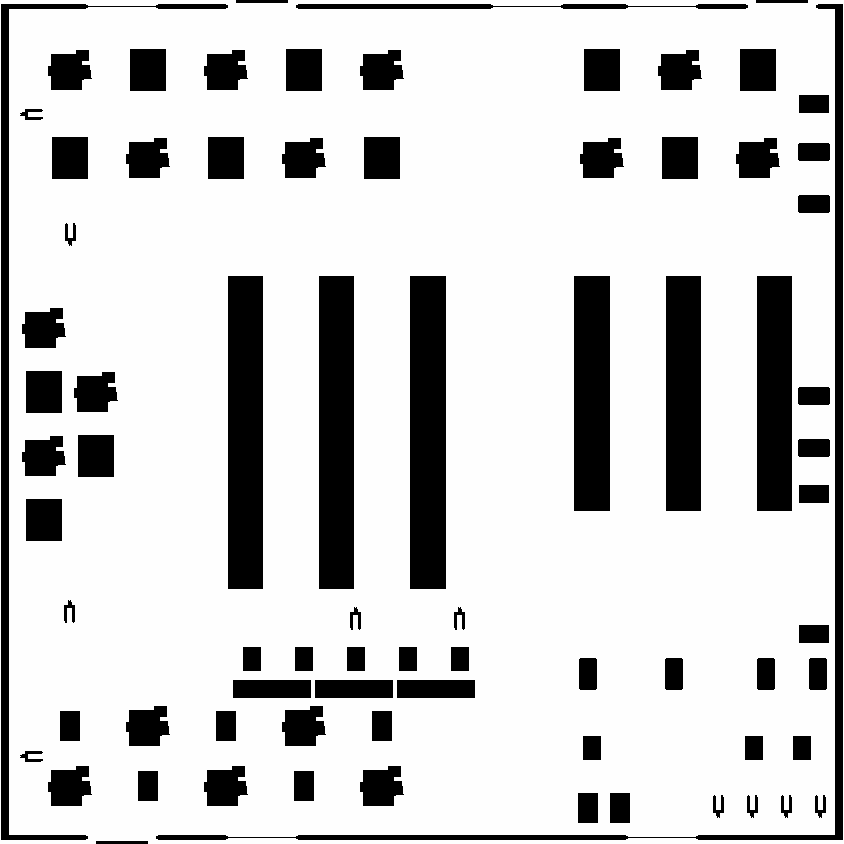
\includegraphics[width=\textwidth]{figures/warehouse_realistic_i.png}\\[0.4ex]
    {\footnotesize (b) I-shape, \SI{19.1}{\percent} occupied}
  \end{minipage}
  \caption[Baked occupancy truth of the two realistic worlds, same frame and resolution as the earlier arrangements.]{Baked occupancy truth of the two realistic worlds, in the frame of
  \cref{fig:warehouse-maps}: \SI{42.2}{\metre} square at \SI{0.05}{\metre} per
  cell, origin $(-21.1,-21.1)$~m. Carriers and loads are baked at their $t=0$
  pose. Closed dock doors are the one-cell segments in the north (and, in~(b),
  south) wall; open doors are the gaps.}
  \label{fig:realistic-maps}
\end{figure}

\begin{queried}[Visual verification]
The generator-side checks are complete, and the first Gazebo session on
6 October 2026 found and fixed one defect the checks could not see (a jack
setting its load down and then stopping on the neighbouring cell, because the
drop command carried one angle for both the parked load and the approach
heading). Three things remain to be confirmed by eye in the simulator rather
than by the checker: that the loads ride on the fork side of the jack, the
shading of the generated door, trailer and yard meshes, and the open/closed
state of each door. Until then the worlds are \status{implemented} in geometry
and \status{partial} in visual verification.
\end{queried}

\paragraph{First recording.} One dataset has been recorded in the family,
\repo{dataset/dataset_map_realistic} (8 October 2026), shown in
\cref{fig:scene-map-realistic} and summarised in \cref{tab:map-realistic}. It
is the first recording outside the \repo{dataset_allsensor} set to carry the
proprioceptive topics, so the baseline of \cref{sec:proprio-method} can be
computed on it, and its median speed of \SI{1.38}{\metre\per\second} is the
closest any simulation recording comes to the \SI{1.5}{\metre\per\second} of
\cref{sec:problem-scope}. The route is a single anticlockwise loop: down the dock lane,
west along cross-aisle C, south through aisle A, east along cross-aisle E and
north between the picking racks and the east wall, ending in dispatch staging.

\begin{figure}[htbp]
  \centering
  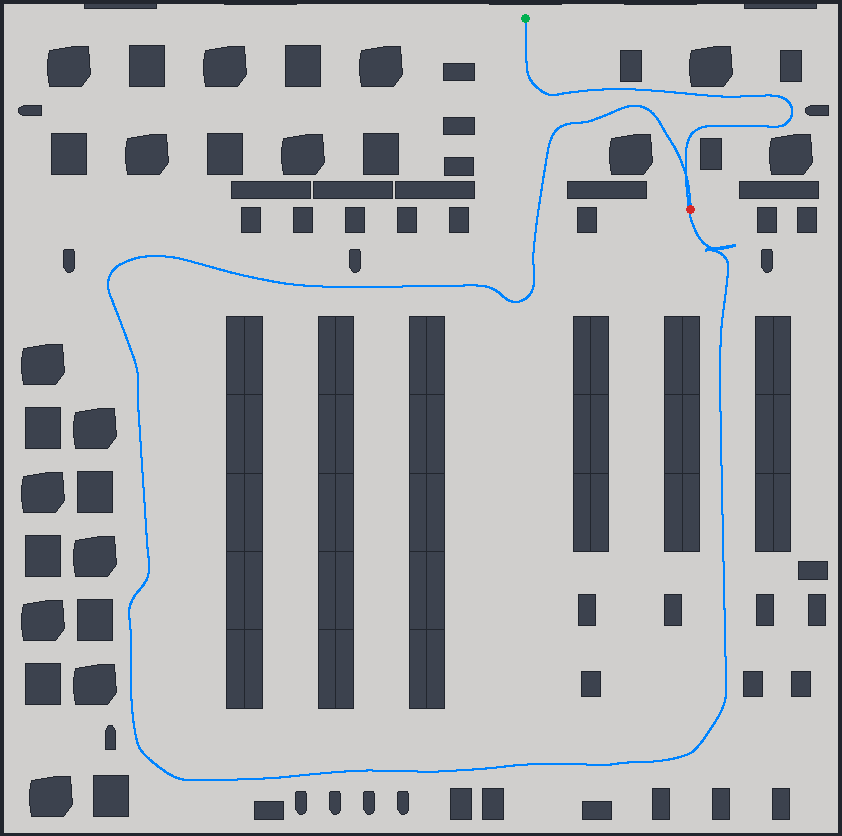
\includegraphics[width=0.62\textwidth]{figures/scene_map_realistic.png}
  \caption[Scene of \repo{dataset_map_realistic}: the U-shape realistic layout and the recorded ground-truth route.]{Scene of \repo{dataset_map_realistic}, drawn with the conventions of
  \cref{fig:dataset-scenes}: obstacle footprints at robot height over the plain
  floor, the \repo{/ground_truth/odometry} route in blue from the green start
  to the red end. The objects are drawn from the U-shape static twin, the world
  the bag's own model inventory identifies (see the query below).}
  \label{fig:scene-map-realistic}
\end{figure}

\begin{table}[htbp]
\centering
\caption[What \repo{dataset_map_realistic} contains, read from the bag.]{What \repo{dataset_map_realistic} contains, read from the bag's
SQLite store rather than its \repo{metadata.yaml}, following
\cref{sec:dataset-registry}. The simulator ran below real time, so the
simulated span is shorter than the recording's wall-clock duration.}
\label{tab:map-realistic}
\small
\begin{tabular}{ll}
\toprule
Quantity & Value \\
\midrule
Recorded & 8 October 2026, \SI{166.5}{\second} wall clock, \SI{126.9}{\second} simulated \\
World & U-shape realistic layout, props stationary (see query) \\
Floor & plain (\texttt{nofloortexture}) \\
Ground-truth route & \SI{151.1}{\metre}, 6\,347 samples, start $(5.25, 20.0)$~m \\
Speed & median \SI{1.38}{\metre\per\second}, 95th percentile \SI{1.51}{\metre\per\second} \\
Images & 3\,847 compressed stereo pairs \\
IMU & 25\,387 messages \\
Proprioception & 126\,938 joint states, 6\,347 wheel-odometry messages \\
\repo{/clock} & present (126\,942 messages) \\
Run manifest & \flag{none} \\
\bottomrule
\end{tabular}
\end{table}

\begin{queried}[Provenance]
\repo{dataset_map_realistic} was recorded without a run manifest, so its
world is not recorded anywhere. It was identified from the bag itself: the
\repo{/world/default/pose/info} stream names 129 models whose numbering and
composition match the regenerated U-shape world and no other, and every model
except the robot holds the same pose from the first message to the last. That
is consistent with the static twin, but also with the dynamic world loaded
without its traffic plugin, and the bag cannot tell the two apart. The exact
\texttt{.world} file must be confirmed by the operator and a manifest written
before the recording is used in any result slot; the identification above is
evidence, not provenance.
\end{queried}
